\section{Method}
\label{method}
Measuring the structure of value creation by individuals is nearly impossible in most in open collaboration projects, in particular when they do not involve writing software code, which can be compiled, executed and tested on computers. Like in Wikipedia, the most common way to code knowledge is natural language (e.g., English, Chinese, Spanish, French, German), which can hardly be systematically tested for performance. Natural language is indeed the realm of subjective interpretation by humans. Here, we present a method to model value creation and performance in such environments, which neither relies on the content nor on subjective metrics, such as the number of edits, or the number of bytes changed overall or per edit. We recognize that value can be brought by each editor, regardless of the frequency, or the length of her contributions. Only the number and the expertise of editors bring value to an article.  And the expertise of editors can be measured from the number and the quality of articles they have modified at least once.

For that, we consider a simple input, which is a representation of the bi-partite network of editors and their contributions to articles.  Namely, let us consider a matrix $M_{ea} \equiv M$ of all editors having contributed to a category of articles on Wikipedia. $M_{ea}$ takes value $1$ if editor $e$ has edited article $a$, and $0$ otherwise. Note that $M$ only shows which editors have ever touched an article. For the category {\it Feminist Writers}, as presented on Figure \ref{fig:triangle}, $M$ exhibits a triangular structure in which editors (resp. articles) are sorted (max on the bottom-left corner) by the number of articles they have touched (resp. by the number of editors who have touched each article). $M$ is the only input of the {\it bi-partite random walker} model described thereafter, for recursively characterizing the structure and the value of contributions in open collaboration, through the evaluation of editors expertise and articles quality.

\begin{figure*}[!t]
\centering
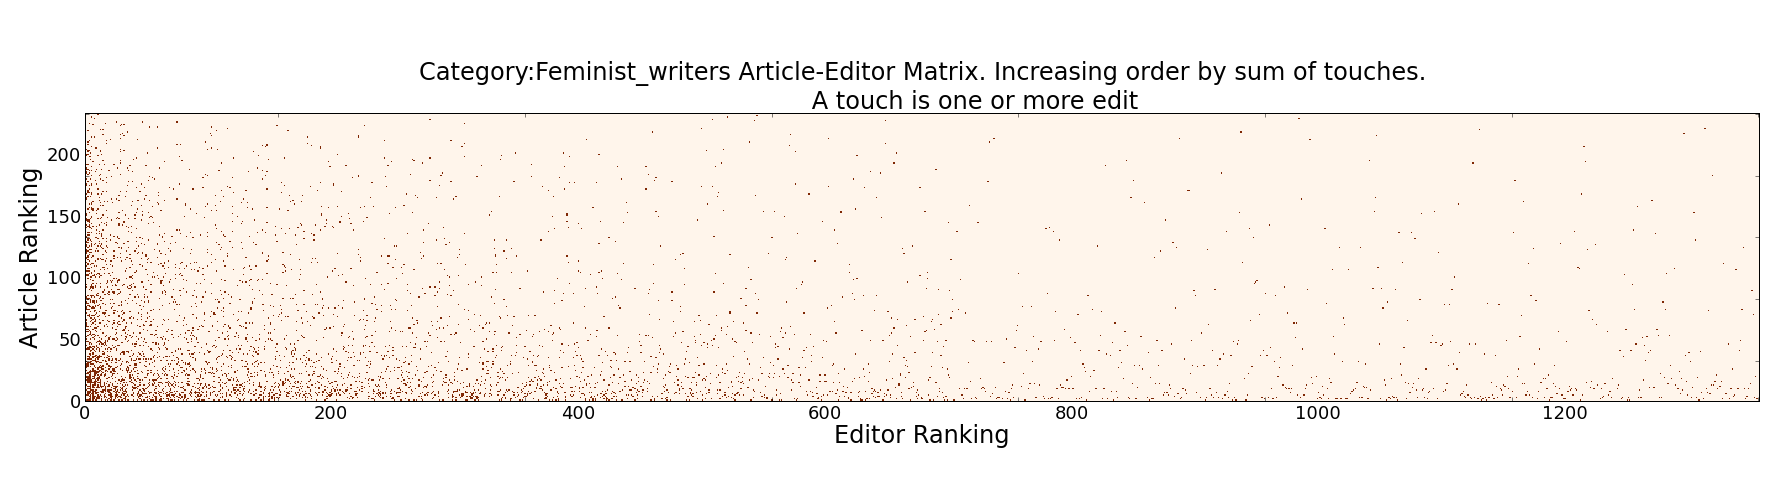
\includegraphics[width=2.0\columnwidth]{../Figures/Category_Feminist_writerstriangle_matrix_corrected.png}
\caption{Typical $\mathbf{M}$ matrix for a Wikipedia category (here, {\it Feminist Writers}) ordered on both dimensions by descending order of number of articles modified by an editor (horizontal axis) and of number editors who have modified an article (vertical axis). The structure of $\mathbf{M}$ is triangular and shows that some editors have a pervasive activity over articles, while most editors edit only a few. Similarly, some articles receive widespread attention by editors, while most articles are modified only by a few editors.}
\label{fig:triangle}
\end{figure*}


Given $M$, the simplest way to assess the contribution value, the {\it expertise}, of an editor is obtained by summing the number of articles ever edited out of a set of articles. Similarly, a simple {\it quality} measure for an article is the sum of editors who have ever modified it, following the famous adage on open source development: ``Given enough eyeballs, all bugs are shallow" \cite{raymond1999}. These crude expertise and quality metrics for editors and articles, respectively  given by,

\begin{equation}
\begin{cases}
 u_{e}^{(0)} = \sum_{a=1}^{N_{a}} M \equiv k_e\\[7pt]
 u_{a}^{(0)} = \sum_{e=1}^{N_{e}} M \equiv k_a,
\end{cases}
\label{HHinit}
\end{equation}

are the zero\textsuperscript{th} order of our algorithm. They are the initial step of the {\it method of reflections} proposed by Hidalgo et al. \cite{hidalgo2007,hidalgo2009}, which derives the value of producing entities (i.e. editors) from products (i.e. articles), and {\it vice versa}. To help capture the intuition behind the method of reflections for open collaboration, we walk through the first and second iterations, as they are adapted to our study of Wikipedia:

\begin{itemize}
  \item {\bf 1\textsuperscript{st} order iteration,}  
  \begin{itemize}
  \item {\bf Articles}: If an article has been edited by higher expertise editors, it is of higher quality. That is, quality is a function of expertise calculated from zero\textsuperscript{th} iteration expertise scores.
  \item {\bf Editors}: Conversely, if an editor has contributed to higher quality articles, her expertise is higher. That is, expertise is a function of quality calculated from zero\textsuperscript{th} iteration quality scores.
  \end{itemize}
  \item {\bf 2\textsuperscript{nd} order iteration,}
    \begin{itemize}
  \item {\bf Articles}: If an article has been changed by higher expertise editors who have edited higher value articles, which in turn have been edited by higher expertise contributors, the article quality is higher. That is, quality is a function of expertise calculated from 1\textsuperscript{st} iteration expertise scores.
  \item {\bf Editors}: Conversely, if an editor has edited higher quality articles, which have been edited by better editors who have edited higher quality articles, then expertise is higher. That is, expertise is a function of quality calculated from 1\textsuperscript{st} iteration quality scores.
  \end{itemize}
 \item {\bf And so on, recursively.}\\
\end{itemize}

Although interpretation is difficult past the very first iteration steps, at each iteration, the algorithm incorporates additional information on the quality of the articles and expertise of editor from the neighboring nodes in the bi-partite network. The higher order iterations of the method of reflections are written as,

\begin{equation}
\begin{cases}
 u_{e}^{(n+1)} = \frac{1}{k_{e}}\sum_{a=1}^{N_{a}} M \, u_{a}^{n}\\[7pt]
 u_{a}^{(n+1)} = \frac{1}{k_{a}}\sum_{e=1}^{N_{e}} M \, u_{e}^{n}.\\
\end{cases}
\label{HHhigher}
\end{equation}

The method of reflections however suffers from a problem, which is rooted in the equal weights given to article and editor scores obtained at the previous iteration. As a result, the method converges to a fixed point with all editors (resp. all articles) having the same value, as a case of consensus dynamics \cite{caldarelli2012network}. It has therefore been proposed to consider giving variable weights to the scores from the previous iteration as a Markov process of random walkers on a bi-partite network, jumping with some probability from one node type to another node type \cite{caldarelli2012network}. A schematic representation of the random walk process on a bi-partite network is depicted in Figure \ref{fig:jumpers}. The intuition is the following: a random walker jumps with some probability from an editor to a given article (i.e. the editor's expertise is positively influenced by the article's quality), and with another probability from an article to a given editor (i.e. the value of the article is positively by the editor's expertise). The matrix $M$ determines whether a jump between each pair of nodes is possible. If two nodes $e$ and $a$ are not directly connected $M_{ea} = 0$, and the transition probability is 0. Conceptually, the {\it bi-partite network random walker} model is an extension of the single node type (i.e. Web pages) {\it Page Rank} Google search algorithm \cite{page1999pagerank} to two kind of nodes.

\begin{figure}[!t]
\centering
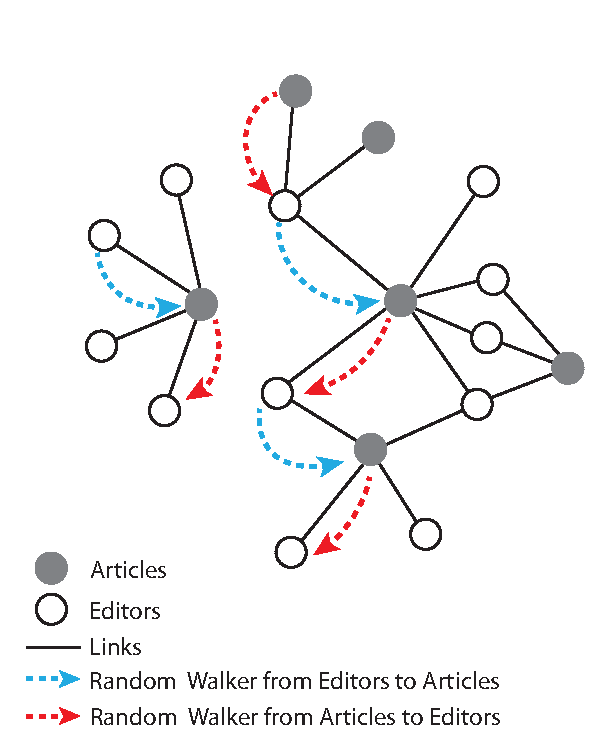
\includegraphics[width=0.7\columnwidth]{../Figures/bi-partite_net.eps}.
\caption{Representation of random walkers jumping from editors to articles (red dotted arrows) and from articles to editors (blue dotted arrows). The intuition is the following: a random walker jumps with some probability from an editor to a given article (i.e. the editor's expertise is positively influenced by the article's quality), and with another probability from an article to a given editor (i.e. the value of the article positively influences the editor's expertise).}
\label{fig:jumpers}
\end{figure}

According to  Caldarelli et al. \cite{caldarelli2012network}, we reformulate the method of reflections to account for jumps of the random walker on the bi-partite network of editors and articles. We call $w^{(n)}_e$ the expertise of an editor and $w^{(n)}_a$ the quality of an article at the $n^{th}$ iteration. We define the following Markov process on the bi-partite network of collaboration, 

\begin{equation}
\begin{cases}
w^{(n+1)}_e (\alpha,\beta) = \sum_{a=1}^{N_a}  G_{ea}(\beta) \,w^{(n)}_a (\alpha,\beta)\\[7pt]
w^{(n+1)}_a (\alpha,\beta) = \sum_{e=1}^{N_e}  G_{ae}(\alpha) \, w^{(n)}_e (\alpha,\beta),\\
\end{cases}
\label{random_walker}
\end{equation}

with $G_{ea}$ the probability  to jump from article $a$ to editor $e$ in a single step, and the probability $G_{ae}$ to jump from editor $e$ to article $a$ also in a single step. These transition probabilities are given by,

\begin{equation}
\begin{cases}
G_{ea}(\beta) = \frac{M_{ea} k_{e}^{-\beta}}{\sum_{e' = 1}^{N_e} M_{e'a} k_{e'}^{-\beta}}\\[10pt]
G_{ae}(\alpha) = \frac{M_{ea} k_{a}^{-\alpha}}{\sum_{a' = 1}^{N_a} M_{ea'} k_{a'}^{-\alpha}}.\\
 \end{cases}
\end{equation}

The transition matrices $G_{ea}(\beta)$ and $G_{ae}(\alpha)$ depend only on the initial conditions: the binary matrix $M$, as well as $k_e$ and $k_a$ given by (\ref{HHinit}). The variables $\alpha$ and $\beta$ control the transition probabilities in a similar way. We shall therefore explain only how $\beta$ influences the probability to jump from an article to an editor (i.e. the value of the article positively influences the editor's expertise). For $\beta = 0$, we recover the zero\textsuperscript{th} order iteration (\ref{HHinit}). For $\beta > 0$, the probability to jump from article $a$ to editor $e$ is a power law function $\sim 1/k_{e}^{\beta}$ of the sum of articles $k_{e}$  modified by editor $e$. Hence, the larger $k_{e}$, the lower the probability to jump from $a$ to $e$ relative to other editors. On the contrary, if $\beta < 0$ the probability to jump from an article to an editor is a positive function of the sum of articles modified by the editor. For $-1 < \beta < 0$, the function is concave, while for $\beta < -1$, the function is convex, which means that the more articles have been edited by the editor, the even more the positive influence on articles. In a nutshell, $\beta$ relates the amount of articles edited on the overall editor's expertise, which in turn has an influence on each edited article (along with the influence of other editors). If $\beta >> 0$, the positive influence of the number of contributed articles on the editor's expertise decreases. If $\beta$ close to $0$, the number of contributed articles increases linearly the editor's expertise. The same considerations hold for $\alpha$ and the probability $G_{ae}(\alpha)$ to jump from an editor to an article (i.e. the expertise of the editor positively influences the quality of an article).

After each iteration, we have expertise and quality scores, which allow ranking editors and articles. When the rankings for both editors and articles do not change in two successive iterations we consider that the {\it bi-partite network random walker} model has converged. We have verified that the method converges on all our 12 Wikipedia categories.  Figure \ref{fig:convergence} shows the evolution of expertise $w_e$ ranked among editors having contributed to articles in the {\it Feminist Writers} category on Wikipedia for arbitrary control parameters: $(\alpha,\beta) =(-0.5, 0.5)$. Starting from the sum of contributed articles as the initial step, we can see how the algorithm progressively ranks editors: some editors with initial low rank (i.e. with few articles edited), get a higher rank as the number of iterations increases. They most probably have edited and contributed to few, but high quality articles. Similarly, some initially high ranked editors, gradually drop in the ranking. They have edited many, but low quality articles. In the case of category {\it Feminist Writers}, the algorithm converges with clearly stable ranks, after nearly $50$ iterations.

\begin{figure}[!t]
\centering
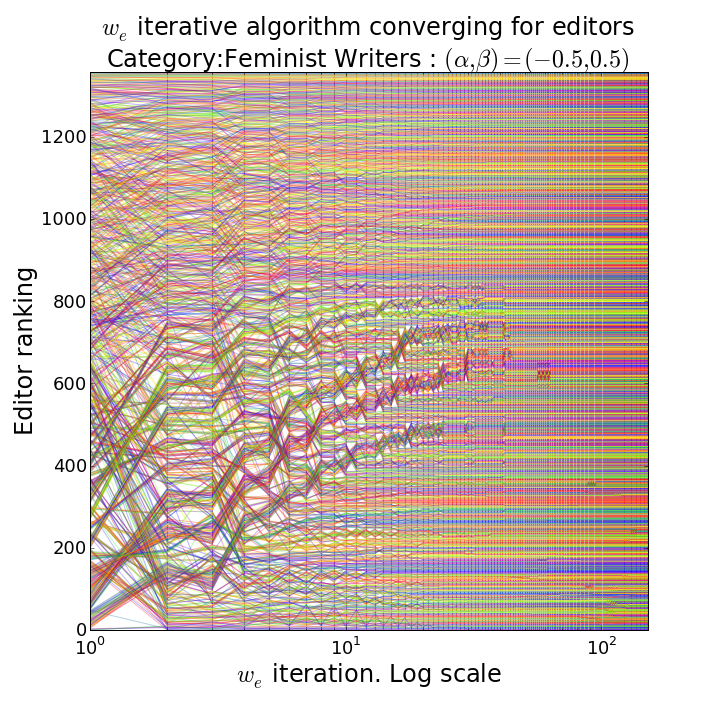
\includegraphics[width=0.9\columnwidth]{../Figures/fem_editors_iter_converge.png}.
\caption{Convergence of the ranked expertise $w_e$ of editors having contributed to articles in the Feminist Writers category on Wikipedia for arbitrary control parameters: $\mathbf{(\alpha,\beta) =(-0.5, 0.5)}$. Starting from the sum of contributed articles as the initial step, we can see how the algorithm progressively ranks editors: some editors with initial lowest rank, i.e. with few articles edited, get a higher rank as the number of iterations increases. Similarly, some initially high ranked editors, gradually drop in the ranking. In the case Wikipedia categories, the algorithm converges with clearly stable ranks, after nearly $\mathbf{50}$ iterations.}
\label{fig:convergence}
\end{figure}


The parameters $\alpha$ and $\beta$ control how editors and articles influence each others at the level of the whole bi-partite collaboration network. Upon calibration with ground-truth editor expertise and article quality metrics, these control parameters thus directly inform on the structure of peer-production, and how contributions benefit to the whole open collaboration project. 

%Whenever calibration shows that the evolution of $\alpha$ and $\beta$ can be predicted, then editors expertise and articles quality can also be predicted up to statistical errors. 
%Here, we explain the calibration steps for$\alpha$ and $\beta$ and how the control parameters inform on the structure of value creation in open collaboration. We also document the evolution of these parameters as Wikipedia categories get increasingly enriched with new contributions.

%A property of this algorithm, is that with the following balance condition,
%
%\begin{equation}
%\mathbf{G}_{ae} \mathbf{w}^*_e = \mathbf{G}_{ea} \mathbf{w}^*_a
%\end{equation}
%
%which can be rewritten as,
%
%\begin{equation}
%\begin{cases}
%\mathbf{w}^{*}_{e} \sim \mathbf{k}^{1-\beta}_{e} \langle \mathbf{k}_{a}^{-\alpha}\rangle_e \\
%\mathbf{w}^{*}_{a} \sim \mathbf{k}^{1-\alpha}_{a} \langle \mathbf{k}_{e}^{-\beta}\rangle_a
%\end{cases} \label{eqsim}
%\end{equation}
%
%it is the analytical formulation we use onwards. It is important to note a crucial difference in the way we apply the weighted random walk model in the case of open collaboration compared to the countries-products problem. In \cite{caldarelli2012network}, $w^*_p$ is a measure of ubiquity (i.e. dis-quality) because many countries can sell the product, while here $w^*_a$ is also a measure of ubiquity in the sense that many editors have modified the article. In the case of open collaboration, $w^*_a$ is a measure of quality.


